%clear;bibtex main.aux; pdflatex main.tex ; evince main.pdf &

%Vous préparerez un exposé de 25 minutes qui sera suivi d'une séance de questions.
%Au cours de l'exposé vous devrez :
%1. Formuler un rappel bibliographique et la problématique qui vous a été proposée. -> problem statement + bilio
%2. Présenter les solutions explorées, et les solutions proposées. -> to do list + explanations
%3. Préciser l'originalité de votre travail par rapport à l'existant. Mix photo + topo -> 3D -> liver -> histo -> threshold -> ident -> vessel
%4. Montrer les résultats obtenus et préciser votre apport. -> quantitative analysis
%5. Préciser les publications envisagées. -> possible


% * * * * * * * * * * * * * * * * * * * * * * * * * * * * * * * * * * * * * * * Slide

\section[Evaluation]{Evaluation}


\subsection[Presentation]{Presentation}
	\begin{frame}
	\frametitle{Presentation}
		\center \alert{Which evaluation protocol?}
		\begin{block}{Difficulties}
			\begin{enumerate}
				\item Choice of the clustering algorithm
				\item Procedure (contextual information)
				\item Data (e.g. noise, brightness, region)
			\end{enumerate}		
		\end{block}\vspace{1em}

		\begin{alertblock}{Evaluation}
			\begin{enumerate}
				\item \emph{K-Means} clustering	% Reduction of polluting data : improving efficiency
				\item Synthetic images % Reduction of data volume : CPU time saving
				\item Benefits of knowledge %Algorithm parameterization 
				\begin{enumerate}
					\item[-] Reduction of polluting data and volume
					\item[-] \emph{K-Means} parameterization 
					%\item[-] Number of cluster
					%\item[-] Centroid
				\end{enumerate}
				%\item Class ordering : algorithm parameterization 
			\end{enumerate}		
		\end{alertblock}

%		\begin{columns}[c]	
%			\column{15em}	
%				
%			\column{15em}
%				\begin{exampleblock}{Expected benefits}
%					\begin{enumerate}
%						\item Increasing of useful data percentage
%						\item Processing time saving
%						\item Setting of thresholding algorithms
%						\item Fewer iterations during the segmentation
%					\end{enumerate}		
%				\end{exampleblock}
%		\end{columns}
	\end{frame}


% * * * * * * * * * * * * * * * * * * * * * * * * * * * * * * * * * * * * * * * Slide

	\subsection[Clustering]{Clustering algorithm}
		\begin{frame}
			\frametitle{Clustering algorithm}	
			\setbeamercovered{invisible}		
			\begin{center}
				\alert{Study limited to only one clustering algorithm to illustrate each benefits.}	
			\end{center}
			\begin{block}{K-Means}
				\begin{enumerate}
					\item A widely used clustering algorithm \textit{``the simplicity and computational speed of the K-means algorithm [...] has made it a popular choice''}\footnotemark[1]
					\item Initialization parameters ($k$, centroid) \textit{``the algorithm needs initializing values which greatly influence its terminating optimal solution ... good initialization is crucial for finding globally optimal partitionings''} \footnotemark[1]
				\end{enumerate}
			\end{block}
			\pause
			\begin{columns}[c]	
			\column{3em}
				\framebox{\includegraphics[trim= 0mm 0mm 0mm 0mm, clip, width=1.0\textwidth]{image/me_4_img_2_no_label.png}}
				\column{0.1em}
				$\Rightarrow$
				\column{8em}
				\multiinclude[format=png,graphics={scale=0.2}]{image/me_4_hist_1}\vspace{1em}
				\column{0.1em}
				$\Rightarrow$
				\column{8em}
				\framebox{\includegraphics[trim= 0mm 0mm 0mm 0mm, clip, height=0.9\textwidth]{image/me_4_0_point.png}}		
			\end{columns}			
%			\begin{center}
%					\alert{Number of classes from inference engine = 3}
%			\end{center}
			\footnotetext[1]{ \tiny \cite{Ranjan2010} Anna D. Peterson Ranjan Maitra and Arka P. Ghosh.
, A systematic evaluation of different methods for initializing the k-means clustering algorithm, \emph{Computer Methods and Programs in Biomedicine}, 2010 }
		\end{frame}
				
% * * * * * * * * * * * * * * * * * * * * * * * * * * * * * * * * * * * * * * * Slide

	\subsection[Polluted data]{Reduction of polluting data and volume}
		\begin{frame}
		\frametitle{ROI + number of classes $\Rightarrow$ reduction of polluting data and volume}
  		%\setbeamercovered{dynamic}
		\setbeamercovered{invisible}

		\begin{columns}[c]	
		\column{9em}
			\framebox{\includegraphics[trim= 0mm 0mm 0mm 0mm, clip, height=1.0\textwidth]{image/me_1_0_img_1.png}}\\
			\begin{center}
				4 classes
			\end{center}				
			\column{0.1em}
			$\Rightarrow$
			\column{12em}
			\multiinclude[format=png,graphics={scale=0.2}]{image/me_1_0_hist_1}\vspace{1em}
			\column{0.1em}
			D
			$\Rightarrow$
			\column{9em}
			\framebox{\includegraphics[trim= 0mm 0mm 0mm 0mm, clip, height=1.0\textwidth]{image/me_1_0_bin_1.png}}		
		\end{columns}\vspace{1em}
		\pause
		\begin{columns}[c]	
		\column{9em}
			\begin{center}		
				\framebox{\includegraphics[trim= 0mm 0mm 0mm 0mm, clip, height=1.0\textwidth]{image/me_1_0_img_2.png}}\\
				2 classes
			\end{center}				
			\column{0.1em}
			$\Rightarrow$
			\column{12em}
			\multiinclude[format=png,graphics={scale=0.2}]{image/me_1_0_hist_2}
			\column{0.1em}
			D
			$\Rightarrow$
			\column{9em}
			\begin{center}					
				\framebox{\includegraphics[trim= 0mm 0mm 0mm 0mm, clip, height=1.0\textwidth]{image/me_1_0_bin_2.png}}			
			\end{center}			
		\end{columns}
		\begin{center}
			\alert{ROI improve efficiency and save time.}
		\end{center}

	\end{frame}
	
% * * * * * * * * * * * * * * * * * * * * * * * * * * * * * * * * * * * * * * * Slide

	\subsection[Number of classes]{Number of classes}

		\begin{frame}
		\frametitle{Number of classes $\Rightarrow$ K-Means parameterization}
		\begin{exampleblock}{No a priori number of clusters\footnotemark[1]}
		
		\begin{columns}[c]	
			\column{18em}
				\begin{center}
					\includegraphics[trim= 0mm 0mm 0mm 0mm, clip, width=0.8\textwidth]{image/me_3_3in1_1.pdf}
				\end{center}
			\column{18em}
				\begin{center}		
					\includegraphics[trim= 0mm 44mm 0mm 0mm, clip, width=0.8\textwidth]{image/me_3_3in1.pdf}
				\end{center}					
		\end{columns}\vspace{1em}
		
		\end{exampleblock}
		
		\begin{exampleblock}{A priori number of cluster}
		
		\begin{columns}[c]	
			\column{14em}	
			\begin{enumerate}
				\item Computing time saving
				\item Optimal clustering
			\end{enumerate}			
			\column{18em}
				\begin{center}		
					\includegraphics[trim= 0mm 0mm 0mm 109mm, clip, width=0.8\textwidth]{image/me_3_3in1.pdf}
				\end{center}					
		\end{columns}\vspace{1em}				
		\end{exampleblock}
	\footnotetext[1]{	\tiny \cite[Ray - 1999]{Ray1999} S Ray and R H Turi, Determination of number of clusters in k-means clustering
..., \emph{Advances in Pattern
Recognition and Digital Techniques}, 2007 }
		\end{frame}
	
% * * * * * * * * * * * * * * * * * * * * * * * * * * * * * * * * * * * * * * * Slide

	\subsection[Centroid]{Centroid initialization}
		\begin{frame}
		\frametitle{Number of classes + ordering = centroids $\Rightarrow$ K-Means parameterization}
		\setbeamercovered{invisible}
		\begin{columns}[c]	
			\column{6em}			
				\framebox{\includegraphics[trim= 0mm 0mm 0mm 0mm, clip, width=1.0\textwidth]{image/me_4_img-0.png}}\\
				\hfill 5 classes \hfill \vspace{1em}
				\framebox{\includegraphics[trim= 0mm 0mm 0mm 0mm, clip, width=1.0\textwidth]{image/centroid_gp.pdf}}
				%\multiinclude[format=png,graphics={scale=0.3}]{image/me_4_img}
			\column{3.6em}<2->
				\framebox{\includegraphics[trim= 0mm 0mm 0mm 0mm, clip, width=1.2\textwidth]{image/me_4_img___1.png}}\\
				3 classes
			\column{12em}<2->
				%\multiinclude[format=pdf,graphics={scale=0.3}]{image/me_4_hist}
				\includegraphics[trim= 25mm 0mm 0mm 0mm, clip, height=1.2\textwidth]{image/me_4_hist-1.pdf}
		\end{columns}

		\begin{columns}<3->[c]	
			\column{10em}
				\framebox{\includegraphics[trim= 0mm 0mm 0mm 0mm, clip, height=0.8\textwidth]{image/me_4_point_manual_4_168131.pdf}}
			\column{10em}
				\framebox{\includegraphics[trim= 0mm 0mm 0mm 0mm, clip, height=0.8\textwidth]{image/me_4_point_random_4_168405.pdf}}
			\column{10em}
				\framebox{\includegraphics[trim= 0mm 0mm 0mm 0mm, clip, height=0.8\textwidth]{image/me_4_point_random_3_743240.pdf}}
		\end{columns}	
		\pause\pause
		\begin{center}
			\alert{Careful seeding = better clustering}
		\end{center}
		\end{frame}
		
%%%%%%%%%%%%%%%%%%%%%%%%%%%%%%%%%%%%%%%%%%%%%%%%%%%%%%%%%%%%%%%%%%%%%%%%%%%%%%% Section

\section{Application}
	\subsection[Presentation]{Presentation}
		\begin{frame}
			\frametitle{Presentation}
			\setbeamercovered{invisible}
			%\begin{block}{Inference engine}
				\begin{enumerate}
					\item Visualization only : less restrictive than segmentation
					\item Preliminary results for two use cases
					\item Medical image  from IRCAD\footnote{IRCAD : Institut de Recherche contre les Cancers de l'Appareil Digestif} database (ground truth)
				\end{enumerate}				
			%\end{block}
%			\begin{columns}[c]	
%			\column{8em}			
				\begin{center}
					\multiinclude[format=png,graphics={scale=0.2}]{image/vrrender}\vspace{1em}				
					%\framebox{\includegraphics[trim= 0mm 0mm 0mm 0mm	, clip, height=1\textwidth]{image/body}}\\
%					\framebox{\includegraphics[trim= 10mm 15mm 10mm 28mm, clip, width=1\textwidth]{image/int_0_0_0}}\\
%					\center{$t=0$}\vspace{1em}
%					\framebox{\includegraphics[trim= 10mm 15mm 10mm 35mm, clip, width=1\textwidth]{image/dicom_liver}}\\
%					\center{$t=1$}
%					\framebox{\includegraphics[trim= 20mm 25mm 20mm 35mm, clip, height=0.2\textwidth]{image/int_0_0_3}}
%					\framebox{\includegraphics[trim= 21mm 25mm 19mm 35mm, clip, height=1\textwidth]{image/int_0_0_4}}
				\end{center}
			%\alert{TOPO GRAPH REAL NAME patient>lung,liver + PHOTO GRADIAN}
%			\column{0.1em}
%			\end{columns}					
		\end{frame}
		
		
	\subsection[Context]{Context}
		\begin{frame}
			\frametitle{Context}
			%\setbeamercovered{invisible}
			\begin{columns}[c]	
			\column{8em}			
				\begin{center}
					%\framebox{\includegraphics[trim= 0mm 0mm 0mm 0mm	, clip, height=1\textwidth]{image/body}}\\
					\framebox{\includegraphics[trim= 10mm 15mm 10mm 28mm, clip, width=0.8\textwidth]{image/int_0_0_0}}\\
					\center{$t=0$}\vspace{1em}
					\framebox{\includegraphics[trim= 10mm 15mm 10mm 35mm, clip, width=0.8\textwidth]{image/dicom_liver}}\\
					\center{$t=1$}
%					\framebox{\includegraphics[trim= 20mm 25mm 20mm 35mm, clip, height=0.2\textwidth]{image/int_0_0_3}}
%					\framebox{\includegraphics[trim= 21mm 25mm 19mm 35mm, clip, height=1\textwidth]{image/int_0_0_4}}
				\end{center}
			%\alert{TOPO GRAPH REAL NAME patient>lung,liver + PHOTO GRADIAN}
			\column{0.1em}
				$\Rightarrow$
			\column{17em}			
				\begin{exampleblock}{A priori knowledges}
					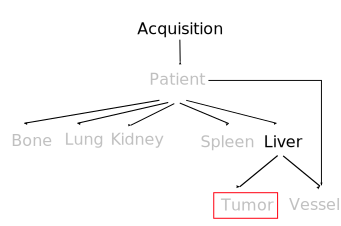
\includegraphics[trim= 0mm 0mm 0mm 0mm	, clip, width=1\textwidth]{image/gt_tumor_label}\\
					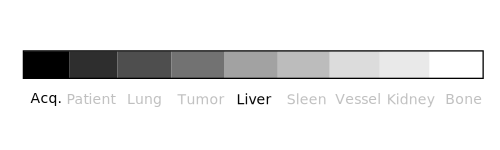
\includegraphics[trim= 0mm 0mm 0mm 0mm	, clip, width=1\textwidth]{image/gp_tumor_label}
				\end{exampleblock}
				\begin{block}{Inference engine}
					\begin{enumerate}
						\item Number of classes = 3
						\item Ordering = tumor < liver < vessel
					\end{enumerate}				
				\end{block}
%			\column{0.1em}
%				$\Rightarrow$				
%			\column{9em}
%				\begin{block}{Clustering}
%					\begin{enumerate}
%						\item Parameterization
%					\end{enumerate}				
%				\end{block}			
%				\begin{center}
%					\framebox{\includegraphics[trim= 0mm 20mm 0mm 15mm, clip, width=1\textwidth]{image/sl_0_3.png}}\vspace{1em}
%					\framebox{\includegraphics[trim= 0mm 10mm 0mm 15mm, clip, width=1.0\textwidth]{image/im_1_4_tumor_rendering_manual.png}}
%				\end{center}
			\end{columns}					
		\end{frame}

% * * * * * * * * * * * * * * * * * * * * * * * * * * * * * * * * * * * * * * * Slide		
		
%	\subsection[How]{How}
%		\begin{frame}
%			\frametitle{How does it works?}
%			\setbeamercovered{invisible}
%			Example with a medical image :\vspace{1em}
%		\begin{columns}[c]
%			\column{13em}
%				\framebox{\includegraphics[trim= 5mm 10mm 3mm 15mm, clip, height=1.0\textwidth]{image/dicom.png}}	
%				\begin{center}
%	%				\alert{Originality: photometric + topologic informations.}
%					\alert{Can you segment the liver?}
%				\end{center}				
%			\column{13em}
%				\framebox{\includegraphics[trim= 5mm 10mm 3mm 15mm, clip, height=1.0\textwidth]{image/dicom_liver.png}}			
%				\begin{center}
%					\alert{Can you segment the tumors?}
%				\end{center}
%		\end{columns}\vspace{1em}
%		\end{frame}
		
% * * * * * * * * * * * * * * * * * * * * * * * * * * * * * * * * * * * * * * * Slide
	\subsection[Use case : tumor]{Use case : tumor}
		\begin{frame}
			\frametitle{Clustering and windowing for tumor}
			\setbeamercovered{invisible}
		\begin{columns}[c]
			\column{8em}	
				\framebox{\includegraphics[trim= 5mm 0mm 3mm 20mm, clip, width=1\textwidth]{image/liver}}
			\column{20em}			
				\multiinclude[format=png,graphics={scale=0.2}]{image/medical_hist}\vspace{1em}
		\end{columns}\vspace{1em}
	
			\begin{center}
				Windowing for \textcolor{MyGreen}{tumor}
			\end{center}\vspace{1em}
		\begin{columns}[c]
			\column{10em}			
				%\framebox{\includegraphics[trim= 5mm 10mm 3mm 15mm, clip, height=1.0\textwidth]{image/liver.png}}
				\framebox{\includegraphics[trim= 5mm 10mm 3mm 15mm, clip, height=1.0\textwidth]{image/im_1_4_tumor_rendering_kmean.png}}
%			\column{0.1em}
%				$\Rightarrow$
			\column{10em}
				\framebox{\includegraphics[trim= 5mm 10mm 3mm 15mm, clip, height=1.0\textwidth]{image/im_1_4_tumor_rendering_manual.png}}
		\end{columns}\vspace{1em}
			
		\end{frame}		

% * * * * * * * * * * * * * * * * * * * * * * * * * * * * * * * * * * * * * * * Slide

	\subsection[Use case : vessel]{Use case : vessel}
		\begin{frame}
			\frametitle{Clustering and windowing for vessel}
			\setbeamercovered{invisible}
		\begin{columns}[c]
			\column{8em}	
				\vspace{1em}
				\framebox{\includegraphics[trim= 5mm 3mm 0mm 10mm, clip, width=0.9\textwidth]{image/im_3_0_render_all}}
			\column{20em}			
				\includegraphics[trim= 0mm 0mm 0mm 0mm, clip, height=0.45\textwidth]{image/medical_vessel_windowing}
		\end{columns}\vspace{2em}
			\begin{center}
				Windowing for \textcolor{red}{vessel}
			\end{center}\vspace{1em}
		\begin{columns}[c]
			\column{10em}			
				\framebox{\includegraphics[trim= 5mm 10mm 3mm 15mm, clip, height=1.0\textwidth]{image/im_3_0_render_vessel_kmean.png}}
			%\column{8em}
				%\framebox{\includegraphics[trim= 5mm 10mm 3mm 15mm, clip, height=1.0\textwidth]{image/im_3_0_render_vessel_1_sigma.png}}
			\column{10em}
				\framebox{\includegraphics[trim= 5mm 10mm 3mm 15mm, clip, height=1.0\textwidth]{image/im_3_0_render_vessel_manual.png}}
		\end{columns}\vspace{1em}
			
		\end{frame}		
%%%%%%%%%%%%%%%%%%%%%%%%%%%%%%%%%%%%%%%%%%%%%%%%%%%%%%%%%%%%%%%%%%%%%%%%%%%%%%% Section

%\section{Analyse}
%	\begin{frame}
%		\frametitle{frame5}
%	\end{frame}

%%%%%%%%%%%%%%%%%%%%%%%%%%%%%%%%%%%%%%%%%%%%%%%%%%%%%%%%%%%%%%%%%%%%%%%%%%%%%%%% Section

%\section[Perspectives]{Perspectives et ameliorations}
%	\begin{frame}
%		\frametitle{frame5}
%	\end{frame}
	
%%%%%%%%%%%%%%%%%%%%%%%%%%%%%%%%%%%%%%%%%%%%%%%%%%%%%%%%%%%%%%%%%%%%%%%%%%%%%%% Section

\section{Conclusion}
	\begin{frame}
		\frametitle{Conclusion}
		\begin{block}{Results}
			\begin{enumerate}
				\item	Generic method for image understanding
				\item	Non quantitative $\Rightarrow$ adaptability
				\item	Constraints:
				\begin{enumerate}
					\item	Perfectly segmented masks
					\item	Complete graph completion			
				\end{enumerate}
			\end{enumerate}
		\end{block}
		\begin{block}{Refinements}
			\begin{enumerate}
				\item	$N$ type value to handle multiplicity and optionality
				\item	Node fully included by successors
			\end{enumerate}
		\end{block}
%		\begin{block}{Prospect}
%			\begin{enumerate}
%				\item	Perfectly segmented masks
%				\item	Graph completion				
%				%\item	
%			\end{enumerate}
%		\end{block}
		
		\begin{block}{Personal}
			\begin{enumerate}
				\item Very pleasant job (research, tools)
				\item Formalization is not easy
				\item The best part just started
			\end{enumerate}
		\end{block}
	\end{frame}


% * * * * * * * * * * * * * * * * * * * * * * * * * * * * * * * * * * * * * * *
% * * * * * * * * * * * * * * * * * * * * * * * * * * * * * * * * * * * * * * *	

